

\section{Independent Component Analysis (ICA) Model}
\label{sec:format}
 

\begin{figure}[t]
\centering
\subfigure{
\includegraphics[height=3.8in,width=5.5in]{chap4/res_7/framework.eps}
}
\caption
{ICA Model. IC1: Independent component containg the foreground text, IC2: Independent
conponent containing the Background IC3; Independent component conating the mixture of foreground and background.
y $\in$ $\{$R,G,B$\}$}
\label{fig:frame}
\end{figure}
Independent Component Analysis (ICA) has been an active research topic 
because of its potential applications in signal processing. And recently 
it has received attention in image processing tasks.
In ICA model, more than one observation signals are needed to achieve the 
analysis.
Currently when ICA is applied in image processing, images are divided into blocks \cite{chap4-1,chap4-2,chap4-3}  
with size of 8x8 or 16x16. These blocks are taken as the observations of ICA model.
But here we divide the image into sub-components i.e Red, Green and blue channels which are
taken as the observation of ICA model(Fig \ref{fig:frame}). 

The goal of ICA is to separate independent 
source signals from the observed signals, which is assumed 
to be the linear mixtures of independent source components. 
The mathematical model of ICA is formulated by 
mixture processing and an explicit decomposition processing.  
Assume there exists a set of `n' unknown source signals 
$S=\{s_1, s_2,..., s_n \}$. The assumptions of the components 
$\{s_i\}$  include mutual independence, stationary and zero mean. 
A set of observed signals $X=\{x_1,x_2,...,x_n\}$, are regarded as the mixture of the source 
components. The most frequently considered 
mixing model is the linear instantaneous noise free model,
which is described as: 
\begin{equation}
x_i=\sum_{j=1}^{n}a_{ij}s_j 
\end{equation}or in the matrix notation
\begin{equation}
X=A.S  
\end{equation}where A is an unknown full rank mixing matrix, which is 
also called mixture matrix. Eqn.1 assumes that there exists a 
linear relationship between the sources $S$ and the observations 
$X$. The ICA model describes how the observed data is 
generated by a process of mixing the components. In our case, `n' is equal to 3. 


\section{Natural Scene Text Binarization}
Understanding texts from natural scenes/scene text image 
such as, commercial signboards, traffic signs, and advertising 
billboards is very useful in many purposes such as assistant 
system for impaired persons, drawing attention of a driver to 
traffic signs, text translation system for foreigners, potential 
applications like license plate recognition, digital note taking, 
document archiving and wearable computing. Binarization 
problem concerns classifying individual pixels as text or 
background. Binarization is necessary to bridge the gap 
between localization and recognition by OCR. The output of 
this step is a binary image where black text characters appear 
on a white background. Current techniques are categorized into 
two groups: global binarization and local binarization or 
adaptive binarization.

Natural scene texts contain numerous degradations not
usually present in machine printed ones such as uneven
lighting, blur, complex background, perspective distortion,
multiple colours etc
% Ctrl - D comments multiple lines & Ctrl - shift - D uncomments it.
In this paper we describe a new algorithm for scene text
segmentation by exploiting inverse rendering, i.e. decomposing
an input image into basic rendering elements. This technique
assigns each pixel in the image to a foreground (text) layer
or a background layer. Previous work [1] has shown that
accurate segmentation can significantly increase the success of
the subsequent text recognition step. However, segmentation in
natural images i because of effects such
as highlights, reflections, shadows, noise and focal blur which can severely degrade the
segmentation accuracy.
Binarization is a process to convert a color or gray scale 
image into blank and white image. It is done to divide the 
image into foreground and background pixels so that text 
extraction can easily perform.  
%In the recent years, content-based image analysis techniques have received more attention with the advent of various digital image capture devices.
%The images captured by these devices can vary dramatically depending on lighting conditions, reflections, shadows and specularities.
%These images contain numerous degradations such as uneven lighting, complex background, multiple colours, blur etc.
%We propose a method for removing reflections, shadows and specularities in natural scene text images and extracting out the text from a single image. 
	
%Binarization method is one of the important pre-processing steps in document image analysis system. 
%It directly affects the performance of the subsequent steps like character/word segmentation and recognition.
%Binarization of text can be defined as classifying individual pixels as foreground (text) or background. 

%There are many algorithms that aim at extracting foreground text from background in images but thresholding remains one of
%the oldest form that is used in many image processing applications. Many sophisticated approaches often have thresholding as a pre-processing step. 
%It is often used to segment images consisting of bright objects against dark backgrounds or vice versa \cite{A1,A3,A4}.
%It typically works well for images where the foreground and background are clearly defined.
%For color thresholding images, most algorithms convert the 
%RGB image into grayscale but here we will make use of the RGB channel as three different sources. 

%Traditional thresholding based binarization can be grouped into two categories: the one which uses global
%threshold for the given images like Otsu \cite{A2}, Kittler {\em et al}. 
%\cite{A5} and the one with local thresholds like Sauvola \cite{A6},
%Niblack \cite{A9}. In global thresholding methods \cite{A2,A7}, global thresholds are
%used for all pixels in image. These methods are fast and robust as
%they use a single threshold based on the global histogram of the gray-value pixels of the image.
%But they are not suitable for complex
%and degraded scene images. 
%Also selecting the right threshold for the whole image is usually a challenge 
%because it is difficult for the thresholding
%algorithm to differentiate foreground text from complex background.
\begin{figure}[t]
\centering
\subfigure[]{

\includegraphics[height=.6in,width=1.7in]{results/res_3/1.eps}

\includegraphics[height=.6in,width=1.7in]{results/res_3/2.eps}

\includegraphics[height=.6in,width=1.7in]{results/res_3/6.eps}
\label{fig:subfig11}
}
\subfigure[]{
\includegraphics[height=.6in,width=1.7in]{results/res_3/3.eps}

\includegraphics[height=.6in,width=1.7in]{results/res_3/4.eps}

\includegraphics[height=.6in,width=1.7in]{results/res_3/8.eps}
\label{fig:subfig12}
}
\subfigure[]{

\includegraphics[height=.6in,width=1.7in]{results/res_3/5.eps}

\includegraphics[height=.6in,width=1.7in]{results/res_3/7.eps}

\includegraphics[height=.6in,width=1.7in]{results/res_3/10.eps}
\label{fig:subfig13}
}
\caption
{Some sample word images we considered in this work containing (a) reflective (b) shadowed and (c) specular background}
\label{fig:1}
\end{figure}
\begin{figure}[t]
\centering
\subfigure{
\includegraphics[height=1.8in,width=3.5in]{results/framework.eps}

\label{fig:subfig11}
}
\caption
{Framework for the proposed method}
\label{fig:3}
\end{figure}


%On the other hand, local or adaptive binarization \cite{A8} methods changes the threshold over the image according to local region properties.
%Adaptive thresholding addresses variations in local intensities throughout the image.
%In these methods, a per-pixel threshold is computed based on a local window around each pixel. 
%Thus, different threshold values are used for different parts of the image. 
%These methods are proposed to overcome global binarization drawbacks but they can be sensitive
%to image artifacts found in natural scene text images like shadows, specularities and reflections.
%Mishra {\em et al}~\cite{A16} has recently formulated the problem of binarization as an MRF optimization problem. 
%The method shows superior performance over traditional binarization methods on many images, and we use it as the
%basis for our comparisons. However, their method is sensitive to the initial auto seeding process.
%On the other hand, we propose a method that removes shadows, specularity and reflections and thus produces a clean 
%binary images even for the images with complex background.
\begin{figure*}[t]
\centering
\subfigure[]{

\includegraphics[height=.5in,width=1.8in]{results/res_5/1.eps}

\includegraphics[height=.5in,width=1.8in]{results/res_5/2.eps}
\includegraphics[height=.5in,width=1.8in]{results/res_5/3.eps}
\label{fig:subfig11}
}
\subfigure[]{

\includegraphics[height=.5in,width=1.8in]{results/res_5/4.eps}

\includegraphics[height=.5in,width=1.8in]{results/res_5/5.eps}

\includegraphics[height=.5in,width=1.8in]{results/res_5/6.eps}
\label{fig:subfig12}
}
\subfigure[]{

\includegraphics[height=.5in,width=1.8in]{results/res_5/7.eps}

\includegraphics[height=.5in,width=1.8in]{results/res_5/8.eps}

\includegraphics[height=.5in,width=1.8in]{results/res_5/9.eps}
\label{fig:subfig12}
}
\caption
{Foreground and Background Extracted: (a) Shadowed background and foreground text
(b) Reflective background and foreground text (c) Specular background and foreground text }
\label{fig:2}
\end{figure*}


%The primary issue related to binarizing text from scene images is the presence of complex/textured background. 
%When the background is uneven as a result of poor or non-uniform lighting conditions, the image will not be 
%segmented correctly by a fixed gray-level threshold. These complex background vary dramatically depending on
%lighting, specularities, reflections and shadows. The above methods applied directly to such images
%give poor results and cannot be used in OCR systems. In this paper, 
%we do an ICA based decomposition which enables us to separate text from complex backgrounds containing, reflections,
%shadows and specularities. 
%For binarization, we apply a global thresholding method on the independent components of the image
%and that with maximum textual properties is used for extracting the foreground text. Binarization results show 
%significant improvement in the extraction of text over other methods. Some of the word images that we used 
%for experiments are shown in Fig \ref{fig:1}.

%The remainder of the paper is organized as follows. We discuss the general ICA model in Section 2 followed by
%the detailed binarization process in section 3. We then show the results of the proposed method on a variety
%of images from the ICDAR dataset, followed by the conclusions and potential directions for further improvement.

% In the recent years, content-based image analysis techniques have received more
% attention with the advent of various digital image capture devices.
% The images captured by these devices can vary dramatically depending on 
% lighting conditions, reflections, shadows and specularities.
% These images contain numerous degradations such as uneven
% lighting, complex background,
% multiple colours, blur etc.
% We propose a method for removing reflections, shadows and specularities in natural scene text images
% and extracting out the text from a single image. 
% 
% Binarization method is one of the important pre-processing steps in
% document image analysis system. 
% It directly affects the performance of the
% subsequent steps like character/word segmentation and recognition.
% Binarization of text can be defined as classifying individual pixels as foreground (text) or
% background. 
% 
% There are many algorithms that aim at extracting foreground 
% (text) from background in images 
% but thresholding remains one of the oldest form that is used
% in many image processing applications. Many sophisticated approaches 
% often have thresholding as a pre-processing step. 
% It is often used to segment images consisting 
% of bright objects against dark backgrounds or vice versa \cite{A1,A3,A4}.
% It typically works well for images where the foreground and background are clearly defined.
% For color thresholding images, most algorithms convert the 
% RGB image into grayscale but here we will make use of the RGB channel as three different sources. 
% 
% Traditional thresholding based binarization can be grouped into two categories: the one which uses global
% threshold for the given images like Otsu \cite{A2}, Kittler {\em et al}. 
% \cite{A5} and the one with local thresholds like Sauvola \cite{A6},
% Niblack \cite{A9}. In global thresholding methods \cite{A2,A7}, global thresholds are
% used for all pixels in image. These methods are fast and robust as
% they use a single threshold based on the global histogram of the gray-value pixels of the image.
% But they are not suitable for complex
% and degraded scene images. 
% Also selecting the right threshold for the whole image is usually a challenge 
% because it is difficult for the thresholding
% algorithm to differentiate foreground text from complex background.
% \begin{figure}[t]
% \centering
% \subfigure[]{
% 
\includegraphics[height=.6in,width=1.6in]{results/res_3/1.eps}
% 
\includegraphics[height=.6in,width=1.6in]{results/res_3/2.eps}
% \label{fig:subfig11}
% }
% \subfigure[]{
% \includegraphics[height=.6in,width=1.6in]{results/res_3/3.eps}
% 
\includegraphics[height=.6in,width=1.6in]{results/res_3/4.eps}
% \label{fig:subfig12}
% }
% \subfigure[]{
% 
\includegraphics[height=.6in,width=1.6in]{results/res_3/5.eps}
% 
\includegraphics[height=.6in,width=1.6in]{results/res_3/6.eps}
% \label{fig:subfig13}
% }
% \caption[]
% {Some sample word images we considered in this work containing (a) reflective (b) shadowed and (c) specular background}
% \label{fig:1}
% \end{figure}
% On the other hand, local or adaptive binarization \cite{A8}
% methods changes the threshold over the image
% according to local region properties.
% Adaptive thresholding addresses variations in
% local intensities throughout the image.
% In these methods, a per-pixel threshold is computed
% based on a local window around each pixel. Thus, different
% threshold values are used for different parts of the image. These
% methods are proposed to overcome global binarization drawbacks
% but they can be sensitive
% to image artifacts found in natural scene text images like shadows, specularities and reflections.
% The recently published work by Mishra \emph{et al} \cite{A16} address the problem
% of binarization as an MRF optimization problem. The method shows superior
% performance over traditional binarization methods on many images, but is sensitive to initial
% auto seeding process. On the other hand, we propose a method which removes
% shadows, specularity and reflections and thus produces a clean binary images
% even for the images with complex background.
% 
% \begin{figure*}[t]
% \centering
% \subfigure[]{
% 
\includegraphics[height=.7in,width=2.0in]{results/res_5/1.eps}
% 
\includegraphics[height=.7in,width=2.0in]{results/res_5/2.eps}
% \includegraphics[height=.7in,width=2.0in]{results/res_5/3.eps}
% \label{fig:subfig11}
% }
% \subfigure[]{
% 
\includegraphics[height=.7in,width=2.0in]{results/res_5/4.eps}
% 
\includegraphics[height=.7in,width=2.0in]{results/res_5/5.eps}
% 
\includegraphics[height=.7in,width=2.0in]{results/res_5/6.eps}
% \label{fig:subfig12}
% }
% \subfigure[]{
% 
\includegraphics[height=.7in,width=2.0in]{results/res_5/7.eps}
% 
\includegraphics[height=.7in,width=2.0in]{results/res_5/8.eps}
% 
\includegraphics[height=.7in,width=2.0in]{results/res_5/9.eps}
% \label{fig:subfig12}
% }
% \caption[]
% {Foreground and Background Extracted: (a) Shadowed background and foreground text
% (b) Reflective background and foreground text (c) Specular background and foreground text }
% \label{fig:2}
% \end{figure*}
% 
% The issue related to binarizing text from
% images is the presence of complex/textured background. 
% When the background is uneven as a result of poor or
% non-uniform lighting conditions, the image will not be segmented correctly by a fixed gray-level
% threshold. These complex background
% vary dramatically depending on lighting, specularities, reflections and shadows.
% The above methods applied directly to these images give poor results and cannot be used 
% in OCR systems. In this paper, an ICA based approach is used as a preprocessing step to 
% extract foreground text from complex backgrounds containing reflections.
% For binarization, we apply a global thresholding method
% on the independent components containing maximum information about the
% foreground text. Binarization results show 
% great improvement in the extraction of text over other methods.  
% Some of the word images that we used for experiments are shown in Fig \ref{fig:1}
% 
% The remainder of the paper is organized as follows. We discuss the general ICA model in
% Section 2. In section 3, we show the detailed binarization process. In section 4,
% experimental results on ICDAR dataset is reported. We finally conclude the
% work in section 5.




%The objective of ICA is to estimate the source signals by 
%finding an decomposition matrix $H$, which is a permuted version of the inverse of the mixing matrix. 
%The separating procedure 
%for estimating the underlying source signals is:
%\begin{equation}
%Y=H.X 
%\end{equation}
%Therefore we find a linear representation of the observed signals, 
%which can satisfy the assumption of statistical independence. 
%But the obtained linear representation cannot 
%mathematically achieve statistical independence. Thus we
%find components that are as independent as possible. These components are only an 
%approximate of the real source signals.
%\begin{equation}
% Y\approx S
%\end{equation}



\subsection{Binarization process}
\begin{figure*}[t]
\centering
\subfigure[Input]{
\includegraphics[height=.6in, width=1.4in]{results/IC/orig.eps}
\label{fig:subfig11}
}
\subfigure[Red]{

\includegraphics[height=.6in, width=1.4in]{results/IC/R.eps}
\label{fig:subfig12}
}
\subfigure[$IC_1$]{

\includegraphics[height=.6in, width=1.4in]{results/IC/14_1.eps}
\label{fig:subfig11}
}
\subfigure[Binarized $IC_1$]{

\includegraphics[height=.6in, width=1.4in]{results/IC/14_1_binary.eps}
\label{fig:subfig13}
}\\
\hspace*{1.5in}
\subfigure[Green]{

\includegraphics[height=.6in, width=1.4in]{results/IC/G.eps}
\label{fig:subfig13}
}
\subfigure[$IC_2$]{

\includegraphics[height=.6in, width=1.4in]{results/IC/14_2.eps}
\label{fig:subfig12}
}
\subfigure[Binarized $IC_2$]{

\includegraphics[height=.6in, width=1.4in]{results/IC/14_2_binary.eps}
\label{fig:subfig13}
}\\
\hspace*{1.5in}
\subfigure[Blue]{

\includegraphics[height=.6in, width=1.4in]{results/IC/B.eps}
\label{fig:subfig14} } 
\subfigure[$IC_3$]{

\includegraphics[height=.6in, width=1.4in]{results/IC/14.eps}
\label{fig:subfig13}
}
\subfigure[Binarized $IC_3$]{

\includegraphics[height=.6in, width=1.4in]{results/IC/binary.eps}
\label{fig:subfig14} } 
\caption
{(a) Original word image (b),(e),(h) R, G and B channel respectively
(c),(f),(i) Independent Components, (d),(g),(j) Binarized image}
\label{fig:4}
\end{figure*}

A wide variety of ICA algorithms are available in the literature \cite{A11,A12}. These algorithms differ from each other on the
basis of the choice of objective function and selected optimization scheme. Here we use a fast fixed point
ICA algorithm to separate out the text from complex background in images. A Blind Source 
Separation method based on SVD \cite{A10} can also be used. Fig. \ref{fig:3} 
shows the complete framework for the proposed method.

\subsubsection{The Separation Model}

Consider the text image as a mixture of pixels from three different sources
and assume it to be a noiseless instantaneous mixture.
We use a single image i.e its R, G and B channels as three observed signals.
Therfore, we can define that the color intensity at each pixel from these three observed signals
mix linearly to give the resultant color intensity at that pixel.
Denoting these mixture images in row vector form
as $x_r$, $x_g$ and $x_b$, the linear mixing of the sources at a particular pixel $k$ can be
expressed in matrix form as follows:

\begin{equation}
%\resizebox{.91\hsize}{!}{$
\underbrace{\left[ {\begin{array}{c}
{x_r(k)} \\
{x_g(k)} \\
{x_b(k)}
 \end{array} } \right]}_{X}
=
\underbrace{\left[ {\begin{array}{ccc}
a_{11} & a_{12} & a_{13} \\
a_{21} & a_{22} & a_{23} \\
a_{31} & a_{32} & a_{33} \\
 \end{array} } \right]}_{A}
\underbrace{\left[ {\begin{array}{c}
s_1(k)\\s_2(k)\\ s_3(k)
 \end{array} } \right]}_{S}
%$}
\end{equation} where $X$ is an instantaneous linear mixture of source
images at pixel $k$, A is the instantaneous $3$x$3$ square mixing matrix and S
is the source images which add up to form the color intensity 
at pixel $k$.  
The mixed images
in $X$ contain a linear combination of the source
images in $S$. We find the mixing matrix A and sources S using fixed point ICA
algorithm.
Derivation of the algorithm is beyond the scope of this paper.
The reader is encouraged to refer \cite{A11} for this. We summarize the 
fixed point ICA method in Algorithm 1.

\begin{algorithm}[t]
\caption{Fixed Point ICA}
\begin{algorithmic}[1] 
\REQUIRE $X$
\STATE Random initialization of $A$
\STATE $S=A^TX$
\STATE $A^+=Xg(S)^T$
where $g(x)=tanh(x)$ 
\STATE $A=A^+/||A^+||$  
\STATE If not converged, go back to 2.
\ENSURE $A,S$ 
\end{algorithmic}
\end{algorithm} 
%The amount of information contained in each independent component can be visually seen.
From this step, we get three independent sources or components.
Fig. \ref{fig:2} shows the background and the foreground extracted.
%The independent component containing the maximum information about the foreground text
%is used for thresholding.
The resultant independent components for a particular word image can be seen in 
%\ref{fig:3}.
Fig. \ref{fig:4} which shows the independent component free from reflective background 
and containing maximum information of the foreground text.

\subsubsection{Thresholding}

Otsu thresholding \cite{A2} is a well-known algorithm that
determines a global threshold for an image by minimizing 
the within-class variance for the resulting classes (foreground pixels 
and background pixels). This is
done by equivalently maximizing the between-class variance
$\sigma _{B}^{2}(T)$ for a given threshold T:
\begin{equation}
\sigma_{B}^{2}=\alpha_1(T)\alpha_2(T)[\mu_1(T)-\mu_2(T)]^2 
\end{equation}
where $\alpha_i$ denotes the number of pixels in each class, $\mu_i$ denotes 
the mean of each class, and T is the value of the potential threshold. 
We apply this thresholding algorithm on all the three independent components to get the binarized image (Fig. \ref{fig:4}).
We can also apply Kittler \cite{A5} algorithm which is also a global thresholding method.
%\begin{figure}[tp]
%\centering
%\subfigure[]{
%\includegraphics[height=.3in,width=1.5in]{results/res_4/orig.eps}
%}
%\subfigure[]{
%
\includegraphics[height=.3in,width=1.5in]{results/res_4/ic.eps}
%}
%\subfigure[]{
%
\includegraphics[height=.3in,width=1.5in]{results/res_4/otsu.eps}
%}
%\subfigure[]{
%
\includegraphics[height=.3in,width=1.5in]{results/res_4/nib.eps}
%\label{fig:subfig12}
%}
%\caption
%{(a) Text containing specular highlight (b) IC (c) Otsu (d) Niblack}
%\label{fig:5}
%\end{figure}
\begin{figure*}[p]
\centering
\subfigure{
\includegraphics[height=.5in,width=1.1in]{chap4/threshold/res1/orig.eps}
\includegraphics[height=.5in,width=1.1in]{chap4/threshold/res1/kit.eps}
\includegraphics[height=.5in,width=1.1in]{chap4/threshold/res1/nib.eps}
\includegraphics[height=.5in,width=1.1in]{chap4/threshold/res1/otsu.eps}
\includegraphics[height=.5in,width=1.1in]{chap4/threshold/res1/sau.eps}
}
\subfigure{
\includegraphics[height=.5in,width=1.1in]{chap4/threshold/res2/orig.eps}
\includegraphics[height=.5in,width=1.1in]{chap4/threshold/res2/kit.eps}
\includegraphics[height=.5in,width=1.1in]{chap4/threshold/res2/nib.eps}
\includegraphics[height=.5in,width=1.1in]{chap4/threshold/res2/otsu.eps}
\includegraphics[height=.5in,width=1.1in]{chap4/threshold/res2/sau.eps}
}
\subfigure{
\includegraphics[height=.5in,width=1.1in]{chap4/threshold/res3/orig.eps}
\includegraphics[height=.5in,width=1.1in]{chap4/threshold/res3/kit.eps}
\includegraphics[height=.5in,width=1.1in]{chap4/threshold/res3/nib.eps}
\includegraphics[height=.5in,width=1.1in]{chap4/threshold/res3/otsu.eps}
\includegraphics[height=.5in,width=1.1in]{chap4/threshold/res3/sau.eps}
}
\subfigure{
\includegraphics[height=.5in,width=1.1in]{chap4/threshold/res4/orig.eps}
\includegraphics[height=.5in,width=1.1in]{chap4/threshold/res4/kit.eps}
\includegraphics[height=.5in,width=1.1in]{chap4/threshold/res4/nib.eps}
\includegraphics[height=.5in,width=1.1in]{chap4/threshold/res4/otsu.eps}
\includegraphics[height=.5in,width=1.1in]{chap4/threshold/res4/sau.eps}
}
\caption
{(a) Image containing Text over another Text (b) Foreground Text (c) Background Text (d)
Text extracted}
\vspace{6mm}
\subfigure{
\includegraphics[height=.5in,width=1.1in]{chap4/threshold/res5/orig.eps}
\includegraphics[height=.5in,width=1.1in]{chap4/threshold/res5/kit.eps}
\includegraphics[height=.5in,width=1.1in]{chap4/threshold/res5/nib.eps}
\includegraphics[height=.5in,width=1.1in]{chap4/threshold/res5/otsu.eps}
\includegraphics[height=.5in,width=1.1in]{chap4/threshold/res5/sau.eps}
}
\subfigure{
\includegraphics[height=.5in,width=1.1in]{chap4/threshold/res6/orig.eps}
\includegraphics[height=.5in,width=1.1in]{chap4/threshold/res6/kit.eps}
\includegraphics[height=.5in,width=1.1in]{chap4/threshold/res6/nib.eps}
\includegraphics[height=.5in,width=1.1in]{chap4/threshold/res6/otsu.eps}
\includegraphics[height=.5in,width=1.1in]{chap4/threshold/res6/sau.eps}
}
\subfigure{
\includegraphics[height=.5in,width=1.1in]{chap4/threshold/res7/orig.eps}
\includegraphics[height=.5in,width=1.1in]{chap4/threshold/res7/kit.eps}
\includegraphics[height=.5in,width=1.1in]{chap4/threshold/res7/nib.eps}
\includegraphics[height=.5in,width=1.1in]{chap4/threshold/res7/otsu.eps}
\includegraphics[height=.5in,width=1.1in]{chap4/threshold/res7/sau.eps}
}
\subfigure{
\includegraphics[height=.5in,width=1.1in]{chap4/threshold/res8/orig.eps}
\includegraphics[height=.5in,width=1.1in]{chap4/threshold/res8/kit.eps}
\includegraphics[height=.5in,width=1.1in]{chap4/threshold/res8/nib.eps}
\includegraphics[height=.5in,width=1.1in]{chap4/threshold/res8/otsu.eps}
\includegraphics[height=.5in,width=1.1in]{chap4/threshold/res8/sau.eps}
}
\caption
{(a) Image containing Text over another Text (b) Foreground Text (c) Background Text (d)
Text extracted}
\label{fig:20}
\end{figure*}
\begin{figure*}[p]
\centering
\subfigure[]{
\includegraphics[height=.5in,width=1in]{chap4/ground/7.eps}
\includegraphics[height=.5in,width=1in]{chap4/ground/8.eps}
\includegraphics[height=.5in,width=1in]{chap4/ground/9.eps}
\includegraphics[height=.5in,width=1in]{chap4/ground/10.eps}
\includegraphics[height=.5in,width=1in]{chap4/ground/11.eps}
}
\subfigure[]{
\includegraphics[height=.5in,width=1in]{chap4/ground/1.eps}
\includegraphics[height=.5in,width=1in]{chap4/ground/2.eps}
\includegraphics[height=.5in,width=1in]{chap4/ground/3.eps}
\includegraphics[height=.5in,width=1in]{chap4/ground/4.eps}
\includegraphics[height=.5in,width=1in]{chap4/ground/5.eps}
}
%\label{fig:subfig11}
\caption
{(a) Image containing Text over another Text (b) Foreground Text (c) Background Text (d)
Text extracted}
\label{fig:20}
\end{figure*}


\begin{figure}[p]
\centering
\subfigure[]{
\includegraphics[height=3.5in,width=5in]{chap4/res_7/pixel_grid.eps}
}
\caption
{(a) Image containing Text over another Text (b) Foreground Text (c) Background Text (d)
Text extracted}
\subfigure[]{
\includegraphics[height=3.5in,width=5in]{chap4/res_7/ocr_recog.eps}
}
\caption
{(a) Image containing Text over another Text (b) Foreground Text (c) Background Text (d)
Text extracted}
\end{figure}
%\begin{figure*}[hbp]
%\centering

%\label{fig:7}
%\end{figure*}

%\begin{figure*}[hbp]
%\centering

%\label{fig:7}
%\end{figure*}








To find the IC that contains the foreground text, we examine the connected components (CC) in the 
binarization of each IC. For each binarized image, we extract the following features from the CCs: 
average aspect ratio, variance of  CC size, and the deviation from linearity of their centroids.
A simple linear classifier is designed to separate the text and non-text classes in the above feature space.
After binarization, we identify the
connected components and remove non-text portions based on size and aspect ratio.

In some cases where the text image is severely degraded and contain different colored text,
adaptive thresholding methods work better and produce good results. As shown in Fig. \ref{fig:5}, adaptive thresholding
method may perform better than global one. However, in practise we note that a simpler global thresholding
scheme works well in most cases.



\subsection{Experimental Results and Analysis}

We used the ICDAR 2003 Robust Word Recognition Dataset \cite{A15} for our experiments.
The dataset contains a set of JPEG images of single words (Sample (171 words), 
TrialTrain (1157 words) and TrialTest (1111 words)). For qualitative evaluation,
we selected the word images that had complex reflective, shadowed and specular background.  
We separate these word images into Red, Green and Blue channels
assuming that these are the mixture images of the independent source images
that contains the foreground (text) and background. These three images are used
for extracting the foreground as described before.

\begin{table}[ht]
\centering
 \caption{Quantitative Results (Average)}
 \scalebox{1.3}{
  \begin{tabular}{| l | c | c | c |}
    \hline
    Method & Precision & Recall & F-score \\ \hline
    Otsu \cite{A2} & .68 & .75 & 69.17 \\ \hline
    Sauvola \cite{A6} & .63 & .81 & 66.94 \\ \hline
    Kittler \cite{A5} & .66 & .76 & 64.33 \\ \hline    
    Niblack \cite{A9} & .70 & .76 & 71.32 \\ \hline   
    MRF \cite{A16} & .79 & .86 & 80.38 \\ \hline
    Proposed &  .86 & .83 & 83.60\\ \hline
  \end{tabular}}
\end{table}
\begin{table}[ht]
\centering
 \caption{OCR Accuracy (\%)}
 \scalebox{1.3}{
  \begin{tabular}{| l | c | c | c |}
    \hline
    Method & Word Accuracy\\ \hline
    MRF \cite{A16} & 43.2 \\ \hline
    Proposed &  61.6\\ \hline
  \end{tabular}}
\end{table}

We compare the performance of our method with four well known thresholding algorithms 
i.e Kittler \cite{A5}, Otsu \cite{A2}, Niblack \cite{A9} and Sauvola \cite{A6}.
We also compare with the recent method by Mishra \emph{et al} \cite{A16}.
It although performs well for many images but severely
fails in cases of shadows, high illumination variations 
in the image. This poor show is likely due to fact that
performance of the algorithm heavily depends on initial seeds.
We show both qualitative and quantitative results of the proposed method. 
The qualitative results are shown in Fig. \ref{fig:6}.
\begin{figure*}[p]
\centering

\subfigure{
\includegraphics[height=.55in,width=1.3in]{results/res_2/1/orig.eps}
\includegraphics[height=.55in,width=1.3in]{results/res_2/1/mrf.eps}
%\subfigure{
%\includegraphics[height=.55in,width=1.2in]{results/res_2/1/kit.eps}
%}
%\subfigure{
%\includegraphics[height=.55in,width=1.2in]{results/res_2/1/otsu.eps}
%}
%\subfigure{
%\includegraphics[height=.55in,width=1.2in]{results/res_2/1/nib.eps}
%}
\includegraphics[height=.55in,width=1.3in]{results/res_2/1/graph.eps}
\includegraphics[height=.55in,width=1.3in]{results/res_2/1/res.eps}
}
%\label{fig:subfig11}
\subfigure{
\includegraphics[height=.55in,width=1.3in]{results/res_2/2/orig.eps}
\includegraphics[height=.55in,width=1.3in]{results/res_2/2/mrf.eps}
%\subfigure{
%\includegraphics[height=.55in,width=1.2in]{results/res_2/2/kit.eps}
%}
%\subfigure{
%\includegraphics[height=.55in,width=1.2in]{results/res_2/2/otsu.eps}
%}
%\subfigure{
%\includegraphics[height=.55in,width=1.2in]{results/res_2/2/nib.eps}
%}
\includegraphics[height=.55in,width=1.3in]{results/res_2/2/graph.eps}
\includegraphics[height=.55in,width=1.3in]{results/res_2/2/res.eps}
}
%\\
%\label{fig:subfig11}
\subfigure{
\includegraphics[height=.55in,width=1.3in]{results/res_2/3/orig.eps}
\includegraphics[height=.55in,width=1.3in]{results/res_2/3/mrf.eps}
%\subfigure{
%\includegraphics[height=.5in,width=1in]{results/res_2/3/kit.eps}
%}
%\subfigure{
%\includegraphics[height=.5in,width=1in]{results/res_2/3/otsu.eps}
%}
%\subfigure{
%\includegraphics[height=.5in,width=1in]{results/res_2/3/nib.eps}
%}
\includegraphics[height=.55in,width=1.3in]{results/res_2/3/graph.eps}
\includegraphics[height=.55in,width=1.3in]{results/res_2/3/res.eps}
}
%\\
%\label{fig:subfig11}
\subfigure{
\includegraphics[height=.55in,width=1.3in]{results/res_2/12/orig.eps}
\includegraphics[height=.55in,width=1.3in]{results/res_2/12/mrf.eps}
%\subfigure{
%\includegraphics[height=.5in,width=1in]{results/res_2/12/kit.eps}
%}
%\subfigure{
%\includegraphics[height=.5in,width=1in]{results/res_2/12/otsu.eps}
%}
%\subfigure{
%\includegraphics[height=.5in,width=1in]{results/res_2/12/nib.eps}
%}
\includegraphics[height=.55in,width=1.3in]{results/res_2/12/graph.eps}
\includegraphics[height=.55in,width=1.3in]{results/res_2/12/res.eps}
}
%\\
%\label{fig:subfig11}
%
%\caption
%{Comparison of Binarization algorithms and the proposed method 
%(From left to right Original, MRF, Kittler, Otsu, Niblack, Sauvola, Proposed)
%Text containing reflective background
%}
%\label{fig:6}
%\end{figure*}
%\begin{figure*}[t]
%\centering
%
\subfigure{
\includegraphics[height=.55in,width=1.3in]{results/res_2/5/orig.eps}
\includegraphics[height=.55in,width=1.3in]{results/res_2/5/mrf.eps}
%\subfigure{
%\includegraphics[height=.5in,width=1in]{results/res_2/5/kit.eps}
%}
%\subfigure{
%\includegraphics[height=.5in,width=1in]{results/res_2/5/otsu.eps}
%}
%\subfigure{
%\includegraphics[height=.5in,width=1in]{results/res_2/5/nib.eps}
%}
\includegraphics[height=.55in,width=1.3in]{results/res_2/5/graph.eps}
\includegraphics[height=.55in,width=1.3in]{results/res_2/5/res.eps}
}
%\\
%\label{fig:subfig11}
\subfigure{
\includegraphics[height=.55in,width=1.3in]{results/res_2/6/orig.eps}
\includegraphics[height=.55in,width=1.3in]{results/res_2/6/mrf.eps}
%\subfigure{
%\includegraphics[height=.5in,width=1in]{results/res_2/6/kit.eps}
%}
%\subfigure{
%\includegraphics[height=.5in,width=1in]{results/res_2/6/otsu.eps}
%}
%\subfigure{
%\includegraphics[height=.5in,width=1in]{results/res_2/6/nib.eps}
%}
\includegraphics[height=.55in,width=1.3in]{results/res_2/6/graph.eps}
\includegraphics[height=.55in,width=1.3in]{results/res_2/6/res.eps}
}
%\\
%\label{fig:subfig11}
%\caption
%{Comparison of Binarization algorithms and the proposed method 
%(From left to right Original, MRF, Kittler, Otsu, Niblack, Sauvola, Proposed)
%Text containing shadowed background
%}
%\label{fig:6}
%\end{figure*}
%\begin{figure*}[t]
%\centering
\subfigure{
\includegraphics[height=.55in,width=1.3in]{results/res_2/7/orig.eps}
\includegraphics[height=.55in,width=1.3in]{results/res_2/7/mrf.eps}
%\subfigure{
%\includegraphics[height=.5in,width=1in]{results/res_2/7/kit.eps}
%}
%\subfigure{
%\includegraphics[height=.5in,width=1in]{results/res_2/7/otsu.eps}
%}
%\subfigure{
%\includegraphics[height=.5in,width=1in]{results/res_2/7/nib.eps}
%}
\includegraphics[height=.55in,width=1.3in]{results/res_2/7/graph.eps}
\includegraphics[height=.55in,width=1.3in]{results/res_2/7/res.eps}
}
%\\
%\label{fig:subfig11}
\subfigure{
\includegraphics[height=.55in,width=1.3in]{results/res_2/8/orig.eps}
\includegraphics[height=.55in,width=1.3in]{results/res_2/8/mrf.eps}
%\subfigure{
%\includegraphics[height=.4in,width=1in]{results/res_2/8/kit.eps}
%}
%\subfigure{
%\includegraphics[height=.4in,width=1in]{results/res_2/8/otsu.eps}
%}
%\subfigure{
%\includegraphics[height=.4in,width=1in]{results/res_2/8/nib.eps}
%}
\includegraphics[height=.55in,width=1.3in]{results/res_2/8/graph.eps}
\includegraphics[height=.55in,width=1.3in]{results/res_2/8/res.eps}
}
%\\
%\label{fig:subfig11}
\subfigure{
\includegraphics[height=.55in,width=1.3in]{results/res_2/9/orig.eps}
\includegraphics[height=.55in,width=1.3in]{results/res_2/9/mrf.eps}
%\subfigure{
%\includegraphics[height=.4in,width=1in]{results/res_2/9/kit.eps}
%}
%\subfigure{
%\includegraphics[height=.4in,width=1in]{results/res_2/9/otsu.eps}
%}
%\subfigure{
%\includegraphics[height=.4in,width=1in]{results/res_2/9/nib.eps}
%}
\includegraphics[height=.55in,width=1.3in]{results/res_2/9/graph.eps}
\includegraphics[height=.55in,width=1.3in]{results/res_2/9/res.eps}
}
%\\
%\label{fig:subfig11}
\subfigure{
\includegraphics[height=.55in,width=1.3in]{results/res_2/10/orig.eps}
\includegraphics[height=.55in,width=1.3in]{results/res_2/10/mrf.eps}
%\subfigure{
%\includegraphics[height=.5in,width=1in]{results/res_2/10/kit.eps}
%}
%\subfigure{
%\includegraphics[height=.5in,width=1in]{results/res_2/10/otsu.eps}
%}
%\subfigure{
%\includegraphics[height=.5in,width=1in]{results/res_2/10/nib.eps}
%}
\includegraphics[height=.55in,width=1.3in]{results/res_2/10/graph.eps}
\includegraphics[height=.55in,width=1.3in]{results/res_2/10/res.eps}
}
%\\
%\label{fig:subfig11}
\subfigure{
\includegraphics[height=.7in,width=1.3in]{results/res_2/11/orig.eps}
\includegraphics[height=.7in,width=1.3in]{results/res_2/11/mrf.eps}
%\subfigure{
%\includegraphics[height=.7in,width=1in]{results/res_2/11/kit.eps}
%}
%\subfigure{
%\includegraphics[height=.7in,width=1in]{results/res_2/11/otsu.eps}
%\includegraphics[height=.7in,width=1in]{results/res_2/11/otsu.eps}
%}
%\subfigure{
%\includegraphics[height=.7in,width=1in]{results/res_2/11/nib.eps}
%}
%\subfigure{
\includegraphics[height=.7in,width=1.3in]{results/res_2/11/graph.eps}
\includegraphics[height=.7in,width=1.3in]{results/res_2/11/res.eps}
}
\label{fig:subfig11}
\caption
{Comparison of Binarization algorithms and the proposed method 
(From left to right Original, MRF, Kittler, Otsu, Niblack, Sauvola, Proposed)
Text containing specular background}
\label{fig:6}
\end{figure*}
We took around 50
images from the dataset and generated its ground truth images for pixel level accuracy.
We use well known measures like precision, recall and F-score to
compare the proposed method with different binarization methods (Table I).
We also use OCR accuracy to show the effectiveness of our method. Note that we are only
using the subset of images that are most degraded by shadowing, illumination variations,
noise and specular reflections. The results of thresholding schemes are too poor for the
OCR algorithm to give any output. Therefore we only compare with the recent MRF~\cite{A16}
based model as shown in Table II.

\begin{figure*}[t]
\centering
\subfigure[]{
\includegraphics[height=.5in,width=1.2in]{results/res_7/1.eps}
}
\subfigure[]{
\includegraphics[height=.5in,width=1.2in]{results/res_7/2.eps}
}
\subfigure[]{
\includegraphics[height=.5in,width=1.2in]{results/res_7/3.eps}
}
\subfigure[]{
\includegraphics[height=.5in,width=1.2in]{results/res_7/4.eps}
\label{fig:subfig11}
}
\caption
{(a) Image containing Text over another Text (b) Foreground Text (c) Background Text (d)
Text extracted}
\subfigure{
\includegraphics[height=.3in,width=1.2in]{results/res_6/1.eps}
\includegraphics[height=.3in,width=1.2in]{results/res_6/2.eps}
\label{fig:subfig11}
}
\caption
{Failure case where both the foreground and background are of same color}
\label{fig:7}
\end{figure*}
The results show that the proposed method is an effective method and performs better than other methods 
in the case where images have
complex background. Fig. \ref{fig:7} shows that our technique can also be applied to text image containing 
two different types of colored text.
We analyze that the above methods do not work in the case where there is a complex and textured background in the images.
It is not that these methods do not work at all. No single algorithm works well for all types of images. Thus we can say
that our method can extract out the text embedded in complex reflective, shadowed and
specular background.
%Though there are some exceptions. Our method does not produce good results when the foreground text and the
%background are of the same color as shown in Fig. \ref{fig:8}.


The failure case of our method is shown in Fig. \ref{fig:8}.
Our method fails in cases where foreground text and the background are of the same color.
Moreover, the approach works only with color images.



% In this section, the results of the proposed method are
% presented. We used ICDAR Robust Word Recognition Dataset \cite{A15}
% for experiments. The dataset contains a set of JPEG images of single words
% (Sample (171 words), TrialTrain (1157 words) and TrialTest (1111 words)).
% We work on the word images that had complex reflective, shadowed and specular background.  
% First, we separate these word images into Red, Green and Blue channels
% assuming that these are the mixture images of the independent source images
% that contains the foreground (text) and background. 
% Then we apply ICA technique to get the independent source images.
% Finally, global thresholding is applied on the component, having maximum information about the foreground text,
% to get the binarize text image.
% 
% We compare the performance of our method with four
% well known thresholding algorithms i.e Kittler \cite{A5},
% Otsu \cite{A2}, Niblack \cite{A9} and Sauvola \cite{A6}. 
% These methods fail to deal with the challenges of scene text images like 
% reflections, shadows and specularities.
% We also compare with the recent method by Mishra \emph{et al} \cite{A16}.
% It although performs well for many images but severely
% fails in cases of shadows, high illumination variations 
% in the image. This poor show is likely due to fact that
% performance of the algorithm heavily depends on initial seeds. 
% 
% 
% We believe a visual evaluation is sufficient for a qualitative estimation of
% our method.
% The results show that the proposed method is an effective
% method and performs better than other methods in the case where images have
% complex background. Fig. \ref{fig:7} shows that our technique can also be applied to text image
% containing two different types of colored text.

%We show both qualitative and quantative results of the proposed method. 
%The qualitative results are shown in Fig. \ref{fig:6}.
%We also use OCR accuracy to show the effectiveness of our method. 
%OCR accuracy for the well known thresholding methods are poor. Therefore
%we only compare with the recent MRF \cite{A16} based model.

%\begin{table}[ht]
%\centering
% \caption{OCR Accuracy (\%)}
% \scalebox{1.3}{
%  \begin{tabular}{| l | c | c | c |}
%    \hline
%    Method & Character Accuracy\\ \hline
%    MRF \cite{A16} & 29.2 \\ \hline
%    Proposed &  50.7\\ \hline
%  \end{tabular}}
%\end{table}


% We analyze that the above methods do not work in the case 
% where there is a complex and textured background in the images.
% It is not that these methods do not work at all. No single algorithm works well for
% all types of images. 
% Thus we can say that our method can extract out the text embedded in complex reflective, shadowed and
% specular background. The failure case of our method is shown in Fig. \ref{fig:8}.
% Our method fails in cases where foreground text and the background are of the same color.



%\begin{figure}[t]
%\centering

%\label{fig:8}
%\end{figure}

\section{Applications}

\subsection{Inscribed Text Segmentation}

\begin{figure}[t]
\centering
\subfigure{
\includegraphics[height=1.5in,width=1.8in]{chap4/res_4/try.eps}
}
\subfigure{
\includegraphics[height=1.5in,width=1.8in]{chap4/res_3/orig.eps}
}
\label{fig:subfig11}
\caption
{Text image where both background and foreground are of same color}
\label{fig:1}
\end{figure}



\begin{figure}[t]
\centering
\subfigure[]{
\includegraphics[height=1.5in,width=1.8in]{chap4/res_2/orig.eps}
}
\subfigure[]{
\includegraphics[height=1.5in,width=1.8in]{chap4/res_2/direct.eps}
}
\subfigure[]{
\includegraphics[height=1.5in,width=1.8in]{chap4/res_2/global.eps}
}
\label{fig:subfig11}
\caption
{(a) Sponge Texture (b),(c) Independent components}
\label{fig:2}
\end{figure}

\begin{figure}[t]
\centering
\subfigure[]{
\includegraphics[height=1.5in,width=1.8in]{chap4/res_1/orig.eps}
}
\subfigure[]{
\includegraphics[height=1.5in,width=1.8in]{chap4/res_1/ica_1.eps}
}
\subfigure[]{
\includegraphics[height=1.5in,width=1.8in]{chap4/res_1/ica_2.eps}
\label{fig:subfig11}
}
\caption
{(a) Image containing text (b),(c) Independent components}
\label{fig:12}
\end{figure}





\begin{figure}[t]
\centering
\subfigure[Original text ]{
\includegraphics[height=1.5in,width=1.6in]{chap4/res_3/orig.eps}
}
\subfigure[Kittler]{
\includegraphics[height=1.5in,width=1.6in]{chap4/res_3/kit.eps}
}
\subfigure[Otsu]{
\includegraphics[height=1.5in,width=1.6in]{chap4/res_3/otsu.eps}
}
\subfigure[Niblack]{
\includegraphics[height=1.5in,width=1.6in]{chap4/res_3/nib.eps}
}
\subfigure[Sauvola]{
\includegraphics[height=1.5in,width=1.6in]{chap4/res_3/sau.eps}
}
\subfigure[ICA + CBM]{
\includegraphics[height=1.5in,width=1.6in]{chap4/res_3/proposed.eps}
}
%\includegraphics[height=.5in,width=1.6in]{chap4/res_1/ica_2.eps}
\label{fig:subfig11}
\caption
{Binarized text}
\label{fig:13}
\end{figure}

\begin{figure}[t]
\centering
\subfigure[Original text ]{
\includegraphics[height=1.3in,width=1.5in]{chap4/res_6/orig.eps}
}
\subfigure[Kittler]{
\includegraphics[height=1.3in,width=1.5in]{chap4/res_6/kit.eps}
}
\subfigure[Otsu]{
\includegraphics[height=1.3in,width=1.5in]{chap4/res_6/otsu.eps}
}
\subfigure[Niblack]{
\includegraphics[height=1.3in,width=1.5in]{chap4/res_6/nib.eps}
}
\subfigure[Sauvola]{
\includegraphics[height=1.3in,width=1.5in]{chap4/res_6/sau.eps}
}
\subfigure[ICA + CBM]{
\includegraphics[height=1.3in,width=1.5in]{chap4/res_6/proposed.eps}
}
%\includegraphics[height=.5in,width=1.6in]{chap4/res_1/ica_2.eps}
\label{fig:subfig11}
\caption
{Binarized text}
\label{fig:13}
\end{figure}
Inscribed text is difficult to extract from one image as both the foregound and the background is of same 
color.
So we capture multiple images and apply our model to extract the text with the help of shadows.
For separating the global and the direct component, we used high frequency checkerboard pattern. 
This takes too much time as we have to capture many images.(Figure \ref{fig:11} shows
the independent component of the sponge texture)
But for this, we apply an Independent Component Analysis (ICA) based method to the images captured containing text.
This method helps in extracting out the shadows(Figure \ref{fig:12}). 
Then we apply our component based model to efficiently binarize the text
embedded (Figure \ref{fig:13}).


\subsection{Enhancing Edge Detection}
Boundary detection is a fundamental task in computer vision, with broad applicability 
in areas such as feature extraction, object recognition and image segmentation. 
The majority of papers on edge detection have focused on using only
low-level cues, such as pixel intensity or color [1{5]. Recent work has started exploring 
the problem of boundary detection based on higher-level representations
of the image, such as motion, surface and depth cues [6{8], segmentation [9], as
well as category specic information [10, 11].

Edge detection refers to the process of identifying and locating sharp discontinuities in an image. The 
discontinuities are abrupt changes in pixel intensity which characterize boundaries of objects in a scene.
Classical methods of edge detection involve convolving the image with an operator (a 2-D filter), which is
constructed to be sensitive to large gradients in the image while returning values of zero in uniform regions.
There are an extremely large number of edge detection operators available, each designed to be sensitive to 
certain types of edges. Variables involved in the selection of an edge detection operator include Edge
orientation, Noise environment and Edge structure. The geometry of the operator determines a characteristic 
direction in which it is most sensitive to edges. Operators can be optimized to look for horizontal, vertical, or 
diagonal edges. Edge detection is difficult in noisy images, since both the noise and the edges contain highfrequency 
content. Attempts to reduce the noise result in blurred and distorted edges. Operators used on noisy 
images are typically larger in scope, so they can average enough data to discount localized noisy pixels.

Boundary detection constitutes a crucial step in many computer vision tasks. A
boundary map of an image can provide valuable information for further image
analysis and interpretation tasks such as segmentation, object description etc.
Fig. 1 shows an image and the associated boundary map as marked by human
observers. It can be noted that the map essentially retains gross but important
details in the image. It is hence sparse yet rich in information from the point
of scene understanding. Extracting a similar boundary map is of interest in
computer vision

Now edges are to be detected from the preprocessed image. 
Conventional edge detection algorithms belong to the high 
pass filtering, which are not fit for complex background 
images. Fixed global threshold will usually work well for 
images with uniform background, but not for textured 
background and the contrast of objects varies within the image 
.In such cases, it is convenient to use a threshold gray level 
that is a slowly varying function of position in the image[14]. 
And also edge continuity to be maintained and edge 
overlapping to be avoided. In this aspect, an iterative 
thresholding algorithm and morphologic erode algorithm [15] 
are used here to detect the edges. Following steps are used to 
detect edges in iterative thresholding
%http://cvit.iiit.ac.in/papers/gopal06AComputational.pdf
%http://vision.ece.ucsb.edu/publications/00edgeflow.pdf
%http://www.cs.cmu.edu/~rahuls/pub/eccv2012-rahuls.pdf

\begin{figure*}[htbp]
\centering
\subfigure{
\includegraphics[height=.7in,width=1.5in]{chap4/edge_detect/15.eps}
\includegraphics[height=.7in,width=1.5in]{chap4/edge_detect/8.eps}
\includegraphics[height=.7in,width=1.5in]{chap4/edge_detect/1.eps}
}
\subfigure{
\includegraphics[height=.7in,width=1.5in]{chap4/edge_detect/16.eps}
\includegraphics[height=.7in,width=1.5in]{chap4/edge_detect/9.eps}
\includegraphics[height=.7in,width=1.5in]{chap4/edge_detect/2.eps}
}
\subfigure{
\includegraphics[height=.7in,width=1.5in]{chap4/edge_detect/17.eps}
\includegraphics[height=.7in,width=1.5in]{chap4/edge_detect/10.eps}
\includegraphics[height=.7in,width=1.5in]{chap4/edge_detect/4.eps}
}
\subfigure{
\includegraphics[height=.7in,width=1.5in]{chap4/edge_detect/18.eps}
\includegraphics[height=.7in,width=1.5in]{chap4/edge_detect/11.eps}
\includegraphics[height=.7in,width=1.5in]{chap4/edge_detect/5.eps}
}
\subfigure{
\includegraphics[height=.7in,width=1.5in]{chap4/edge_detect/21.eps}
\includegraphics[height=.7in,width=1.5in]{chap4/edge_detect/14.eps}
\includegraphics[height=.7in,width=1.5in]{chap4/edge_detect/7.eps}
}
%\label{fig:subfig11}
\caption
{(a) Image containing Text over another Text (b) Foreground Text (c) Background Text (d)
Text extracted}
\label{fig:20}
\end{figure*}
\subsection{Shadow Detection}
Shadows, created wherever an object obscures the light
source, are an ever-present aspect of our visual experience.
Shadows can either aid or confound scene interpretation,
depending on whether we model the shadows or ignore
them. If we can detect shadows, we can better localize objects, 
infer object shape, and determine where objects contact the ground. Detected shadows also provide cues for
lighting direction and scene geometry. On the other
hand, if we ignore shadows, spurious edges on the boundaries of shadows and confusion between albedo and shading

can lead to mistakes in visual processing. For these reasons,
shadow detection has long been considered a crucial component of scene interpretation (e.g., [17, 2]). But despite it
importance and long tradition, shadow detection remains an
extremely challenging problem, particularly from a single
image.
The main dif�?culty is due to the complex interactions of
geometry, albedo, and illumination. Locally, we cannot tell
if a surface is dark due to shading or albedo, as illustrated
in Figure 1. To determine if a region is in shadow, we must
compare the region to others that have the same material and
orientation. For this reason, most research focuses on modeling 
the differences in color, intensity, and texture of neighboring pixels or regions. 
Many approaches are motivated by
physical models of illumination and color [12, 15, 16, 7, 5].

The obstruction of light by objects creates shadows in a scene. An object may cast a 
shadow on itself, called self-shadow. The shadow areas are less illuminated than the 
surrounding areas. In some cases the shadows provide useful information, such as Shadow 
detection and removal is an important pre-processing task in many of the 
computer vision applications. The shadows may give rise to false segments in the 
image segmentation process. Also, shadows may be wrongly detected as objects in 
object detection algorithms. Various pixel-based and region-based methods were 
proposed to detect the shadows in an image. This section briefly reviews some of 
the important research works in shadow detection and removal.
the relative position of an object from the source. But they cause problems in 
computer vision applications like segmentation, object detection and object 
counting. Thus shadow detection and removal is a pre-processing task in many 
computer vision applications. Based on the intensity, the shadows are of two types
hard and soft shadows. The soft shadows retain the texture of the background 
surface, whereas the hard shadows are too dark and have little texture. Thus the 
detection of hard shadows is complicated as they may be mistaken as dark objects 
rather than shadows. 
%http://www.cs.illinois.edu/~dhoiem/publications/cvpr11_shadow.pdf
%http://www.cit.iit.bas.bg/CIT_2013/v13-1/S_Murali,%20V_Govindan.pdf
\begin{figure*}[htbp]
\centering
\subfigure{
\includegraphics[height=.8in,width=1.3in]{chap4/shadow/1.eps}
}
\subfigure{
\includegraphics[height=.8in,width=1.3in]{chap4/shadow/2.eps}
}
\subfigure{
\includegraphics[height=.8in,width=1.3in]{chap4/shadow/3.eps}
}
\subfigure{
\includegraphics[height=.8in,width=1.3in]{chap4/shadow/4.eps}
}
\subfigure{
\includegraphics[height=.8in,width=1.3in]{chap4/shadow/5.eps}
}
\subfigure{
\includegraphics[height=.8in,width=1.3in]{chap4/shadow/6.eps}
}
\subfigure{
\includegraphics[height=.8in,width=1.3in]{chap4/shadow/7.eps}
}
\subfigure{
\includegraphics[height=.8in,width=1.3in]{chap4/shadow/8.eps}
}
\subfigure{
\includegraphics[height=.8in,width=1.3in]{chap4/shadow/9.eps}
}
\subfigure{
\includegraphics[height=.8in,width=1.3in]{chap4/shadow/10.eps}
}
\subfigure{
\includegraphics[height=.8in,width=1.3in]{chap4/shadow/11.eps}
}
\subfigure{
\includegraphics[height=.8in,width=1.3in]{chap4/shadow/12.eps}
}
%\label{fig:subfig11}
\caption
{(a) Image containing Text over another Text (b) Foreground Text (c) Background Text (d)
Text extracted}
\label{fig:20}
\end{figure*}
